\chapter{اولین قدم‌ها با اوبونتو}
در این فصل ما به بررسی کارهای ابتدایی با اوبونتو می‌پردازیم.
\section{آشنایی با اجزای مختلف محیط کاربری}
هنگامی که ما برای اولین بار وارد محیط اوبونتو می‌شویم، محیط رومیزی مانند شکل زیر است.

\begin{figure}[hbtp]
\centering
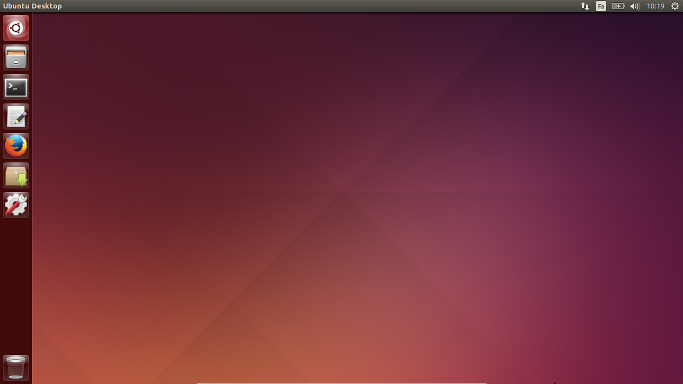
\includegraphics[scale=0.7]{pics/ubuntu-14.04.png}
\caption{محیط رومیزی اوبونتو}
\end{figure}
\subsection{محیط رومیزی}
محیط رومیزی
\footnote{\lr{Desktop Environment}}
پیش‌فرض هنگام نصب اوبونتو، یونیتی
\footnote{\lr{Unity}} 
است. این محیط رومیزی بر پایه‌ی گنوم ۳ کار می‌کند.
\subsection{فایرفاکس}
این مرورگر به صورت پیش‌فرض بر روی اوبونتو نصب می‌باشد.
\subsection{ترمینال}
\subsection{لیبره‌آفیس}
\subsubsection{لیبره‌آفیس رایتر}
\subsubsection{لیبره‌آفیس کلک}
\subsubsection{لیبره‌آفیس ایمپرس}
\section{بروزرسانی}
اولین کاری که می‌توان برای بهبود کارایی سیستم‌عامل انجام داد، به‌روزرسانی سیستم‌عامل است. این امر از طریق‌های متفاوتی قابل انجام است که در این قسمت با استفاده از ترمینال گفته می‌شود.

\begin{latin}
\begin{lstlisting}
$ sudo apt-get update
\end{lstlisting}
\end{latin}

\begin{latin}
\begin{lstlisting}
$ sudo apt-get dist-upgrade
\end{lstlisting}
\end{latin}
\section{نصب نرم‌افزار}
نصب نرم‌افزار در سیستم‌عامل اوبونتو از چند طریق ممکن است. 

\begin{itemize}
\item از طریق نرم‌افزار 
«\lr{Ubuntu Software Center}»
\item از طریق ترمینال و یا
\item از طریق نرم‌افزار \lr{Synaptic Package Manager}.
\end{itemize}

\section{سفارشی سازی محیط رومیزی}
برای سفارشی سازی
\footnote{\lr{customizing}}
محیط رومیزی می‌توان از نرم‌افزار gnome-tweak-tool یا unity-tweak-tool اقدام نمود.

\section{پرسشگان}
\section{مطالعه‌ی بیشتر}
